\documentclass{article}
\usepackage[utf8]{inputenc}
\usepackage[greek,english]{babel}
\usepackage{alphabeta}
\usepackage{fancyhdr}
\usepackage{listings}
\usepackage{mathtools}
\usepackage{xcolor}
\usepackage{biblatex}
\usepackage[left=2cm,right=2cm]{geometry}

\lstset {
        basicstyle=\ttfamily,
        columns=fullflexible,
        breaklines=true,
        keepspaces=true
}

\title{Εργαστήριο Παράλληλου Υπολογισμού - Εργασία 2}
\author{Χρήστος Μαργιώλης}
\date{Ιανουάριος 2020}

\begin{document}

\begin{titlepage}
        \maketitle
\end{titlepage}

\renewcommand{\contentsname}{Περιεχόμενα}
\tableofcontents

\section{Τεκμηρίωση}

Το πρόγραμμα, προκειμένου να υλοποίησει τα ερωτήματα της άσκησης,
ακολουθεί την εξής δομή:
\begin{itemize}
        \item Δέχεται το διάνυσμα $X$ και το μήκος του στον επεξεργαστή 0.
        \item Υπολογίζει τα παρακάτω ωστέ να είναι πιο
                εύκολη και οργανωμένη η υλοποίηση του υπόλοιπου
                προγράμματος.
        \begin{itemize}
                \item $X_{min}$
                \item $X_{max}$
                \item $m$ - Μέση τιμή
                \item \lstinline{scounts} και \lstinline{displs} - Για να
                χρησιμοποιηθούν από τις \lstinline{MPI_Scatterv(3)}
                και \lstinline{MPI_Gatherv(3)}.
                \item Τοπικό $n$ για τον κάθε επεξεργαστή καθώς και το
                διάνυσμα που του αναλογεί.
        \end{itemize}
        \item Αφού γίνουν επιτυχώς τα παραπάνω, υλοποιεί τα ερωτήματα.
        \begin{itemize}
                \item Πόσα στοιχεία είναι μικρότερα ή μεγαλύτερα της μέσης τιμής $m$.
                \item Την διασπορά των στοιχείων του διανύσματος $X$.
                \item Διάνυσμα $Δ$.
                \item Την μεγαλύτερη τιμή του διανύσματος $Δ$ καθώς και την 
                θέση της στο διάνυσμα.
                \item Το διάνυσμα προθεμάτων (prefix sums) των στοιχείων
                του διανύσματος $X$.
        \end{itemize}
        \item Εμφανίζει όλα τα ζητούμενα αποτελέσματα στον επεξεργαστή 0.
\end{itemize}

Αυτό που αξίζει προσοχή είναι οι πίνακες \lstinline{scounts} και
\lstinline{displs} που ανέφερα παραπάνω. Προκειμένου να μοιράζεται σωστά το
διάνυσμα ακόμα και στην περίπτωση που το $n$ δεν είναι ακέραιο πολλαπλάσιο του
$p$, πρέπει να χρησιμοποιηθούνε οι συναρτήσεις \lstinline{MPI_Scatterv(3)} και
\lstinline{MPI_Gatherv(3)} - αυτές οι συναρτήσεις είναι παρόμοιες με τις
\lstinline{MPI_Scatter(3)} και \lstinline{MPI_Gather(3)}, με την διαφορά ότι
μπορούνε να δεχτούνε μεταβλητό αριθμό στοιχείων προς αποστολή στον κάθε επεξεργαστή.
Για παράδειγμα, ας υποθέσουμε ότι είμαστε στην περίπτωση που το $n$ \textit{είναι}
πολλαπλάσιο του $p$ και έχουμε το εξής input:

\[p = 4\]
\[n = 8 \]
\[X = \{1, 2, 3, 4, 5, 6, 7, 8\}\]
Τότε, μπορούμε να ισομοιράσουμε τα στοιχεία στους $p = 4$ επεξεργαστές ως εξής:
\[p_0 = \{1, 2\}\]
\[p_1 = \{3, 4\}\]
\[p_2 = \{5, 6\}\]
\[p_3 = \{7, 8\}\]

Στην περίπτωση όμως που το $n$ \textit{δεν} είναι ακέραιο πολλαπλάσιο του $p$,
χρειαζόμαστε να μοιράσουμε τα στοιχεία έτσι ώστε όλοι οι επεξεργαστές να έχουνε
μέχρι 1 στοιχείο παραπάνω, προκειμένου ο υπολογιστικός φόρτος να είναι όσο το
δυνατόν πιο ίσα μοιρασμένος. Οπότε, έχοντας το παρακάτω input ως παράδειγμα:

\[p = 4\]
\[n = 11 \]
\[X = \{1, 2, 3, 4, 5, 6, 7, 8, 9, 10, 11\}\]
Με βάση τα παραπάνω λεγόμενά μου, τα στοιχεία πρέπει να μοιραστούν ως εξής:
\[p_0 = \{1, 2, 3\}\]
\[p_1 = \{4, 5, 6\}\]
\[p_2 = \{7, 8, 9\}\]
\[p_3 = \{10, 11\}\]

Προκειμένου να επιλυθεί αυτό το πρόβλημα, χρησιμοποιούμε, όπως προανέφερα,
τις συναρτήσεις \lstinline{MPI_Scatterv(3)} και \lstinline{MPI_Gatherv(3)}.
Τα νέα ορίσματα που μάς απασχολούνε είναι τα εξής δύο:

\begin{itemize}
        \item \lstinline{scounts} - αριθμός στοιχείων που παίρνει ο κάθε επεξεργαστής
        \item \lstinline{displs} - offset στο γενικό διάνυσμα
\end{itemize}

Και τα δύο ορίσματα (πίνακες) έχουνε μήκος $p$, ωστέ σε κάθε
θέση του πίνακα να υπάρχουνε οι κατάλληλες πληροφορίες για το πώς θα μοιραστούν
τα στοιχεία στον κάθε επεξεργαστή.

Έπειτα, θέτουμε τις κατάλληλες τιμές για το τοπικό $n$ και διάνυσμα. Στον κώδικα
έχω κάνει \lstinline{localn = scounts[rank]} το οποίο, αν και προφανές, σημαίνει
ότι το κάθε τοπικό διάνυσμα έχει μήκος όσο και τα στοιχεία που υπολογίσαμε ότι
θα έχει ο επεξεργαστής που θα το δεχτεί. Στην συνέχεια στέλνουμε - επιτέλους -
μέσω της \lstinline{MPI_Scatterv(3)} σε όλους τους επεξεργαστές το διάνυσμα που
τούς αναλογεί.

Μετά από τα παραπάνω βήματα, ξεκινάνε οι υπολογισμοί για τα ζητούμενα της άσκησης,
οπότε θα εξήγησω στο επόμενος μέρος περιληπτικά τί κάνει η κάθε συνάρτηση που έχω
υλοποιήσει με την σειρά που εκτελούνται στο πρόγραμμα.

\section{Συναρτήσεις}

\subsection{\lstinline{float input(const char *fmt, int i)}}

Δίνει την δυνατότητα για formatted input.

\subsection{\lstinline{float find(int flag)}} \label{find}

Βρίσκει το $X_{min}$ και $X_{max}$ ανάλογα με το flag που
τής έχει δωθεί. Τα flags που μπορούνε να δωθούν είναι τα εξής
\begin{itemize}
        \item \lstinline{FIND_XMIN}
        \item \lstinline{FIND_XMAX}
\end{itemize}
Προκειμένου να υπολογίσει οποιαδήποτε από τις δύο τιμές ακολουθεί τον
εξής αλγόριθμο:
\begin{itemize}
        \item Για κάθε στοιχείο του τοπικού διανύσματος του εκάστοτε
        επεξεργαστή, βρες το τοπικό μέγιστο ή ελάχιστο.
        \item Μάζεψε τα αποτέλεσματα από όλους τους επεξεργαστές στον
        \lstinline{root}.
        \item Βρες το ολικό μέγιστο ή ελάχιστο με την ίδια λογική όπως
        στο πρώτο βήμα.
        \item Στείλε το αποτέλεσμα σε όλους τους επεξεργαστές.
\end{itemize}

\subsection{\lstinline{float calcavg(void)}} \label{calcavg}

Υπολογίζει την ολική μέση τιμή. Αρχικά βρίσκει όλα τα
τοπικά μέγιστα, τα μαζεύει στον \lstinline{root} επεξεργαστή,
ο οποίος βρίσκει την ολική μέση τιμή και την στέλνει σε
όλους τους υπόλοιπους επεξεργαστές.

\subsection{\lstinline{float findavg(float *v, int len)}}

Βοηθητική συνάρτηση για υπολογισμό μέσης τιμής. Χρησιμοποιείται από την
\lstinline{calcavg} [\ref{calcavg}].

\subsection{\lstinline{int count(float avg, int flag)}}

Υπολογίζει πόσα στοιχεία είναι είτε μεγαλύτερα είτε μικρότερα της ολικής
μέσης τιμής $m$. Το τί από τα δύο θα υπολογίσει εξαρτάται από το flag που
θα τής δωθεί. Τα flags που δέχεται είναι τα εξής:
\begin{itemize}
        \item \lstinline{COUNT_BELOW_AVG}
        \item \lstinline{COUNT_ABOVE_AVG}
\end{itemize}

Για τους υπολογισμούς ακολουθεί παρόμοια λογική με την \lstinline{find} [\ref{find}].

\subsection{\lstinline{float calcvar(float avg)}}

Υπολογίζει την ολική διασπορά των στοιχείων του διανύσματος $X$. Ως όρισμα
δέχεται την μέση τιμή $m$ που υπολογίζει η \lstinline{calcavg} [\ref{calcavg}].
Ο τύπος που χρησιμοποιεί για τον υπολογισμό της τοπικής διασποράς είναι:
\[var_{local} = \sum_{i = 0}^{n_{local}} (x_{i} - m)^2\]
Αφού μαζέψει όλα τα τοπικά αποτελέσματα στον επεξεργαστή \lstinline{root}, 
τα αθροίζει και τα διαιρεί δια $n - 1$, ώστε να ολοκληρωθεί ο τύπος της διασποράς.
\[var = \frac{1}{n - 1} \cdot \sum_{i = 0}^{n - 1} (x_i - m)^2\]

\subsection{\lstinline{float *calcd(float xmin, float xmax)}}

Δημιουργεί ένα νέο διάνυσμα $Δ$, του οποίο το κάθε στοιχείο $δ_i$ είναι ίσο
με 
\[δ_i = ((x_i - x_{min}) / (x_{max} - x_{min})) \cdot 100 \]

Αφού υπολογίσει τον παραπάνω τύπο για κάθε στοιχείο όλων των τοπικών διανυσμάτων,
μαζεύει όλα τα διανύσματα στον επεξεργαστή \lstinline{root} μέσω της
\lstinline{MPI_Gatherv(3)}.

\subsection{\lstinline{Pair findmax(float *d)}}

Βρίσκει το ολικό μέγιστο στο διάνυσμα $Δ$ καθώς και την θέση του στο διάνυσμα.
Αρχικά, αυτό που επιστρέφει η συνάρτηση είναι ένα \lstinline{struct Pair}, το
οποίο είναι ένα \lstinline{struct} που δημιούργησα ώστε να αποθηκεύσω τα δύο
αποτέλεσματα που θα παράξει η συνάρτηση αυτή ($D_{max}$ και $D_{maxloc}$).

Ο αλγόριθμος που ακολουθεί η συνάρτηση είναι ο εξής:
\begin{itemize}
        \item Για κάθε στοιχείο του γενικού διανύσματος $Δ$, ψάξε
        το μέγιστο στοιχείο και την θέση του.
        \item Αφού βρεθεί, με την χρήση της \lstinline{MPI_Reduce(3)},
        βρες την θέση το ολικό μέγιστο καθώς και την θέση του και αποθήκευσέ
        τα στο \lstinline{out} στον επεξεργαστή \lstinline{root}.
\end{itemize}

\subsection{\lstinline{float *calcpfxsums(void)}}

Υπολογίζει το διάνυσμα προθεμάτων (prefix sums) των στοιχείων του
διανύσματος $X$. Προκειμένου να γίνει αυτό χρησιμοποείται η συνάρτηση
\lstinline{MPI_Scan(3)}, η οποία κάνει όλους τους απαραίτητους υπολογισμούς.
Εμείς το μόνο που έχουμε να κάνουμε είναι να αποθηκεύσουμε τα αποτελέσματα στον
πίνακα \lstinline{pfxsums}. Σημαντικό να σημειωθεί ότι αυτή η συνάρτηση
εκτελείται επιτυχώς \textit{μόνο} στην περίπτωση που $n = p$. 

\subsection{\lstinline{void printv(const char *str, const float *v)}}

Βοηθτική συνάρτηση για να τυπώνει διανύσματα με πιο όμορφο τρόπο.

\subsection{\lstinline{void *emalloc(size_t nb)}}

\lstinline{malloc(3)} με error checks.

\section{Κώδικας}
\lstinputlisting[language=C]{ex2.c}

\section{Προβλήματα}

Δεν κατάφερα να βρω πώς να υλοποιηθεί η εύρεση του διανύσματος προθεμάτων
στην περίπτωση που το $n \neq p$.

\section{Ενδεικτικά τρεξίματα}

Input: $p = 4$, $n = 7$, $X = \{1, 2, 3, 4, -1, -2, 6\}$ \\

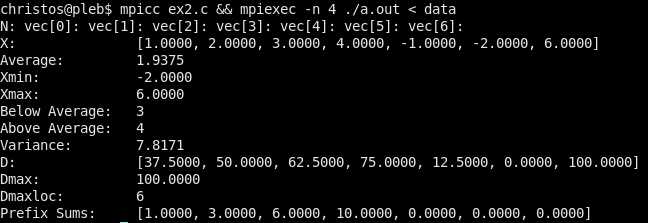
\includegraphics[width=\textwidth]{res/run1.png} \\

Input: $p = 4$, $n = 11$, $X = \{1, 2, -5, 21, 13, 6, -10, 8, 9, 4, -6\}$ \\

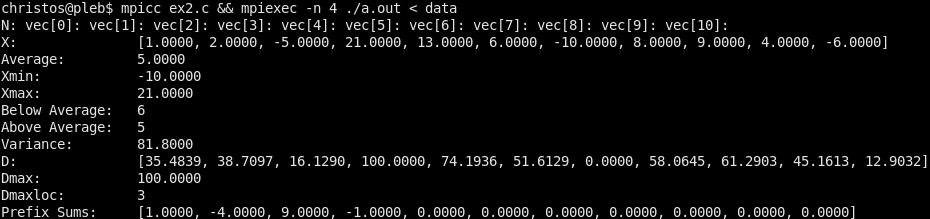
\includegraphics[width=\textwidth]{res/run2.png} \\

Input: $p = 8$, $n = 8$, $X = \{2, 3, 4, 5, 6, -1, -2\}$ \\
Εφόσον τώρα ισχύει $n = p$, η συνάρτηση για την έυρεση των
prefix sums θα λειτουργήσει σωστά. \\

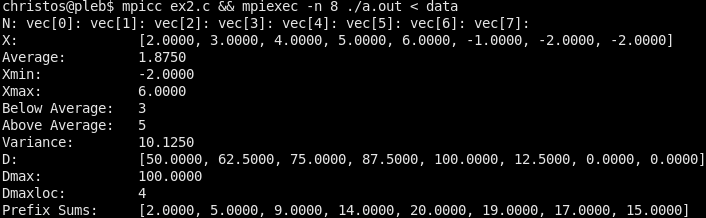
\includegraphics[width=\textwidth]{res/run3.png} \\

\end{document}
